\documentclass{article}
\usepackage{multicol}
\usepackage{hyperref}
\usepackage{graphicx}
\usepackage{caption}
\usepackage{capt-of}
\newenvironment{Figure}
  {\par\medskip\noindent\minipage{\linewidth}}
  {\endminipage\par\medskip}

\title{Forrest Fire Simulation model}
\author{Tom Peerdeman - 10266185 \& Ren\'e Aparicio Saez - 10214054}

\begin{document}

\maketitle

\begin{abstract}
\textbf{Le Abstract.}
\end{abstract}

\begin{multicols}{2}
\subsection*{Introduction}

\subsection*{Core}
\subsubsection*{Different grids and their neighborhoods}
Forest fires can spread in various ways. In order to ensure that the simulation is applicable in many situations, three different types of grids were used to simulate the forest fires on. These grids are: the Cartesian grid, a hexagonal grid and a triangular grid. Each grid has a different spread of fire.\\\\
For the Cartesian grid a straightforward method is used. By using a Moore neighborhood like grid the eight squares around the current square can be directly influenced.\\\\
The hexagonal grid could be positioned in two different ways. Either with flat sides of the hexagon along the y-axis, or with the flat sides along the x-axis. Both types of hexagons will do, by changing your perspective on the simulation, you can simulate the other type of hexagon. For the experiments and simulations the type with sides along the x-axis is chosen.\\\\
Just like the hexagonal grid, the triangular grid can be placed in two different ways. Either along the y-axis or the x-axis. Again, the latter is chosen, to keep consistency for both grids. Whereas the fire spread of the Cartesian and the hexagonal grids are the same, no matter the location, the spread of the triangular grid differs per position. The triangle can either point up or down, switching along each axis.
\begin{Figure}
 \centering
 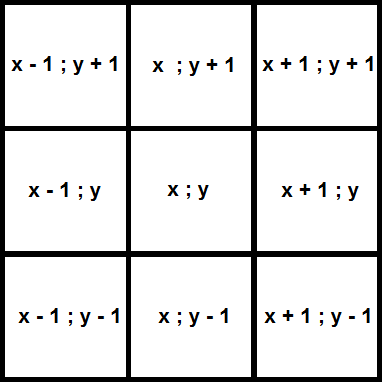
\includegraphics[width=0.79\textwidth]{imgs/cartesian.png}
 \captionof{figure}{Cartesian grid neighborhood}
\label{fig:cartesianstd}
\end{Figure}
\begin{Figure}
 \centering
 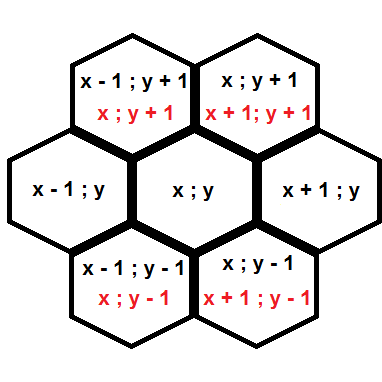
\includegraphics[width=0.79\textwidth]{imgs/hexagonal.png}
 \captionof{figure}{Hexagonal grid neighborhood}
\label{fig:cartesianstd}
\end{Figure}
\begin{Figure}
 \centering
 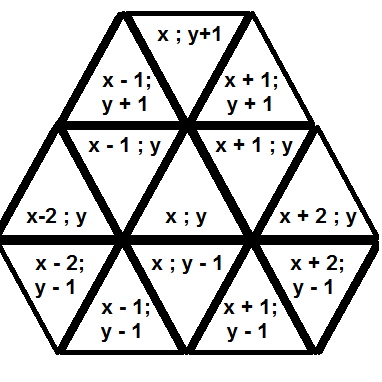
\includegraphics[width=0.79\textwidth]{imgs/triangle1.png}
 \captionof{figure}{Triangle1 grid neighborhood}
\label{fig:cartesianstd}
\end{Figure}
\begin{Figure}
 \centering
 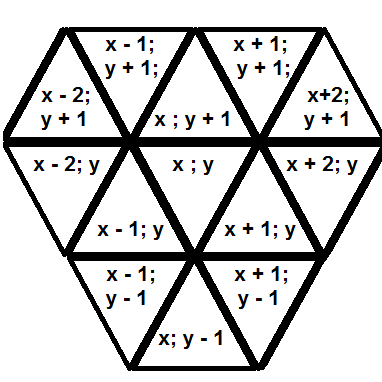
\includegraphics[width=0.79\textwidth]{imgs/triangle2.png}
 \captionof{figure}{Triangle2 grid neighborhood}
\label{fig:cartesianstd}
\end{Figure}

\subsubsection*{Spread probabilities}
Each grid can be initialized with certain probabilities for their neighborhoods. These probabilities stand for the probability of fire to catch on that specific cell, if the current cell is on fire. By using probabilities, instead of just looking if a cell is going to be turned on or off, different types of variables can be used when simulating the fire. By changing the probabilities in certain ways, different types of weather, wind and terrain can be simulated. For example, when the weather is rainy, the probabilities can be set lower, while when it’s hot the probabilities can be set higher. The same goes for wind, if the wind blows in a certain direction, the probabilities for that direction can be set higher than the other directions.\\\\
In order to increase the environmental factor even more, it is also possible to increase the size of the neighborhood. In this way, extreme hot weather or high wind speeds can be simulated even better. When the neighborhood is increased, a new probability is created for fire to catch in a distance of two cells from the current cell. This probability is calculated by dividing the interpolated probabilities for that cell by a given number. This way, the probability for fire to spread is always equal or lower to the values of the cells its probability was interpolated from.
The areas that could be set on fire if the spread of distance two is enabled is shown in the following figures. Note that the area of the triangles is a bit odd. The area that would have been able to get on fire if all the surrounding cells were used, was too big in comparison to the other grids. Because of that the area for the triangles has been reduced.

\subsection*{Experiments}
\subsection*{Results}
\subsection*{Interpretation}

\subsection*{Discussion \& Conclusion}

\subsection*{References}
\end{multicols}
\newpage
\bibliographystyle{plain}
\bibliography{paper}
\end{document}
